\documentclass{article}
\usepackage[utf8]{inputenc}

\usepackage{amsthm}
\usepackage{amsfonts}
\usepackage{amsmath}
\usepackage{amssymb}
\usepackage{fullpage}
\usepackage{graphicx}
\usepackage[usenames]{color}
\usepackage{hyperref}
  \hypersetup{
    colorlinks = true,
    urlcolor = blue,       % color of external links using \href
    linkcolor= blue,       % color of internal links 
    citecolor= blue,       % color of links to bibliography
    filecolor= blue,        % color of file links
    }
    
\usepackage{listings}
\usepackage{textgreek} % added so I could add the epsilon in text
\usepackage{tipa} % added so I could add the pipe symbol |
\usepackage{bussproofs}
\usepackage{multicol} % added to do columns
\usepackage[backend=biber,style=alphabetic,sorting=ynt]{biblatex}
\addbibresource{citations.bib}

\definecolor{dkgreen}{rgb}{0,0.6,0}
\definecolor{gray}{rgb}{0.5,0.5,0.5}
\definecolor{mauve}{rgb}{0.58,0,0.82}

\lstset{frame=tb,
  language=haskell,
  aboveskip=3mm,
  belowskip=3mm,
  showstringspaces=false,
  columns=flexible,
  basicstyle={\small\ttfamily},
  numbers=none,
  numberstyle=\tiny\color{gray},
  keywordstyle=\color{blue},
  commentstyle=\color{dkgreen},
  stringstyle=\color{mauve},
  breaklines=true,
  breakatwhitespace=true,
  tabsize=3
}

\theoremstyle{theorem} 
   \newtheorem{theorem}{Theorem}[section]
   \newtheorem{corollary}[theorem]{Corollary}
   \newtheorem{lemma}[theorem]{Lemma}
   \newtheorem{proposition}[theorem]{Proposition}
\theoremstyle{definition}
   \newtheorem{definition}[theorem]{Definition}
   \newtheorem{example}[theorem]{Example}
\theoremstyle{remark}    
  \newtheorem{remark}[theorem]{Remark}


\title{CPSC-402 Report}
\author{Stephen White}

\date{\today}

\begin{document}

\maketitle

\begin{abstract}
In short, the goal is to search for all occurrences of a small string within a larger string. We are trying to emulate the text searching abilities of Regular Expressions. 
\end{abstract}

\tableofcontents

\section{Introduction}\label{intro}

My name is Stephen White. I am a Computer Science major with a minor in Business Administration at Chapman University.

\section{Homework}\label{homework}

This section contains the solutions to the homework. 

\subsection{Week 1}

%For most weeks, you will have a subsection that contains your answers.

\subsubsection{Homework 1.1}
The homework discussed in this section can be seen \href{https://hackmd.io/@alexhkurz/rycnvMvgu}{here}.
Part 1 of the homework is exercise 2.2.4 item B. The problem can be found on page 54 of the textbook (page 69 of the pdf).
\newline \newline
The first question is as follows: "Give DFA's accepting the following languages over the alphabet \{0,1\}: The set of all strings with three consecutive 0's (not necessarily at the end)."
\newline\newline
My answer to this question is as follows:\\
Since we know that this DFA's alphabet can only consist of 0's and 1's, and we are searching for three consecutive 0's, looking like this: 000, we can formally defined the DFA as 
\begin{align*}
    \{\omega\ |\ \omega\ is\ of\ the\ form\ x000y\ for\ some\ strings\ x\ and\ y\ consisting\ of\ 0's\ and\ 1's\ only \}
\end{align*}

The following image is a diagram of this DFA showing its states and transitions.\\
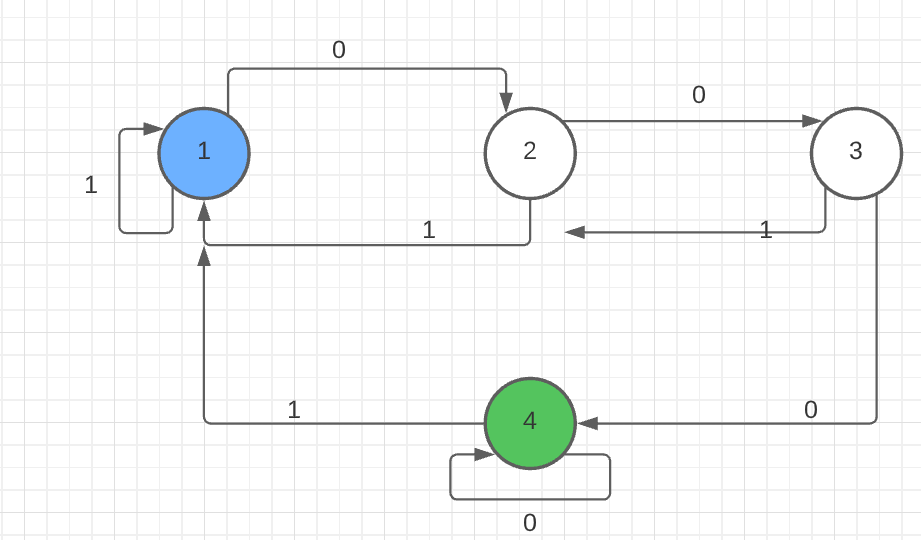
\includegraphics{Question224PartB.png}\\
(I have chosen blue to signify the initial state and green to signify the success state)\\

The next question asks "Give DFA's accepting the following languages over the alphabet \{0,1\}: The set of strings with 011 as a substring."\\\\
My answer to this question is as follows:\\
Since we know that this DFA's alphabet can only consist of 0's and 1's, and we are searching for the string 011, we can formally defined the DFA as 
\begin{align*}
    \{\omega\ |\ \omega\ is\ of\ the\ form\ x011y\ for\ some\ strings\ x\ and\ y\ consisting\ of\ 0's\ and\ 1's\ only \}
\end{align*}

The following image is a diagram of this DFA showing its states and transitions.\\
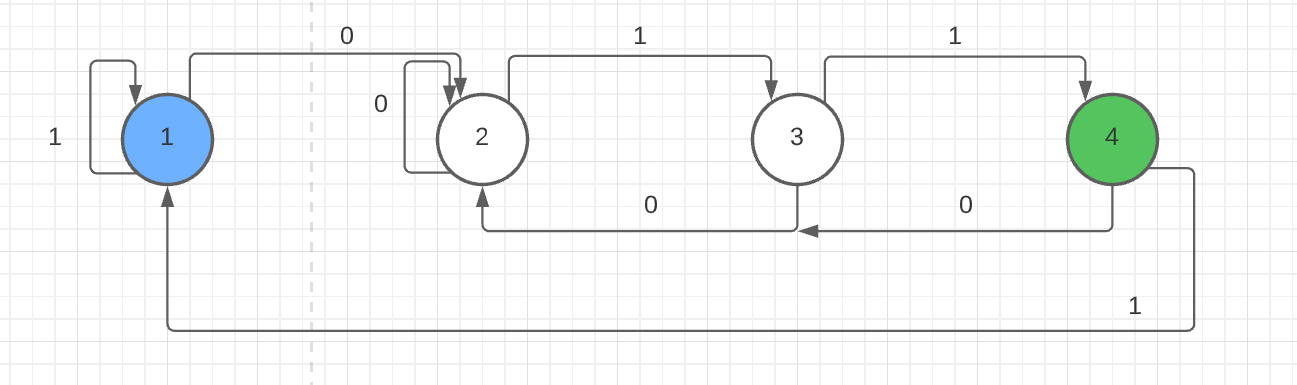
\includegraphics[scale=0.75]{Question224PartC.png}\\
(I have chosen blue to signify the initial state and green to signify the success state)\\

\subsubsection{Homework 1.2}
The homework discussed in this section can be seen \href{https://github.com/alexhkurz/compiler-construction-2022/blob/main/homework-1.2.md}{here}.\\\\

Part 1 of this assignment is to answer the following question: 
\begin{center}
    "Does the file contain the sequence aa or abb? For example, if the file is aaabbaabb, the output should be [2,3,5,7,9]. The challenge here is to not write a program that runs twice through the file, once to search for aa and once for abb, but to find a way of running through the file only once and to simultaneously search for both strings."
\end{center}

I chose to write the program in C\# because I am most familiar with it, and I believe it has a good mix between control and programming speed. That code can be found \href{https://github.com/mamba72/CompilerConstruction_Assignments/blob/main/Reports/ReportResources/StringSearchingImplementation.cs}{here on my GitHub}.
To aid me in my understanding of the problem, I made the following diagram of the DFA I was creating:\\
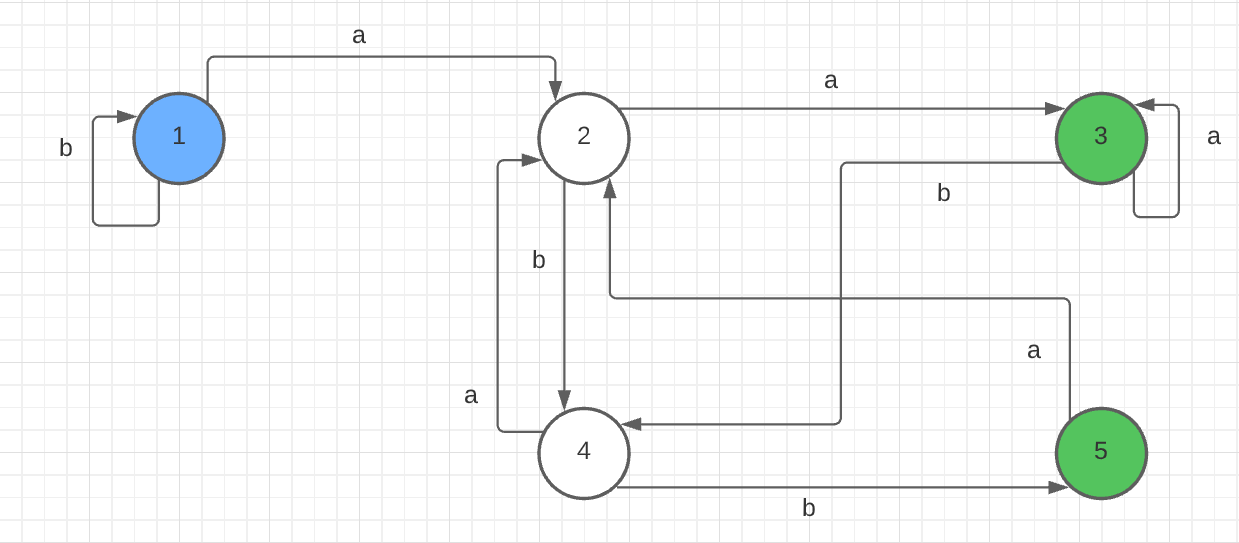
\includegraphics[scale = 0.7]{Question3DFA.png}\\\\

Part 2 of the homework was to complete exercise 2.2.10 (the proof being optional) on page 54 of the textbook (page 70 of the pdf).\\
The question reads as follows:
\begin{center}
    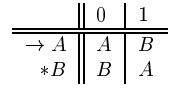
\includegraphics[]{Exercise2210Diagram.png}\\
"Informally describe the language accepted by this DFA."
\end{center}
I tackled this problem by first breaking down the chart, to understand what I was being asked. The chart is similar to a Punnett Square. The left column is a list of the possible current states (an input). The top row is a list of possible character inputs. The rest of the chart is the next state (the output) determined by that row's current state and current character. Since the only possible characters are 1 and 0, the language accepted by this DFA is a set of strings or words created by any combination of 0's and 1's. 


\subsection{Week 2}

\subsubsection{Homework 2.1.1 Composing Automata}
The homework discussed in this section can be found \href{https://hackmd.io/@alexhkurz/ryV_FU7XI}{here}.\\
\textbf{Exercise 2.3.4}\\
Part 1 of this assignment is to answer the following questions:\\
\\
Find NFAs that recognize:\\
\includegraphics[scale=0.3]{Questions 2-3-4.png}\\

\textbf{Part A:}\\
The NFA I created is outlined in the diagram below.
\begin{center}
    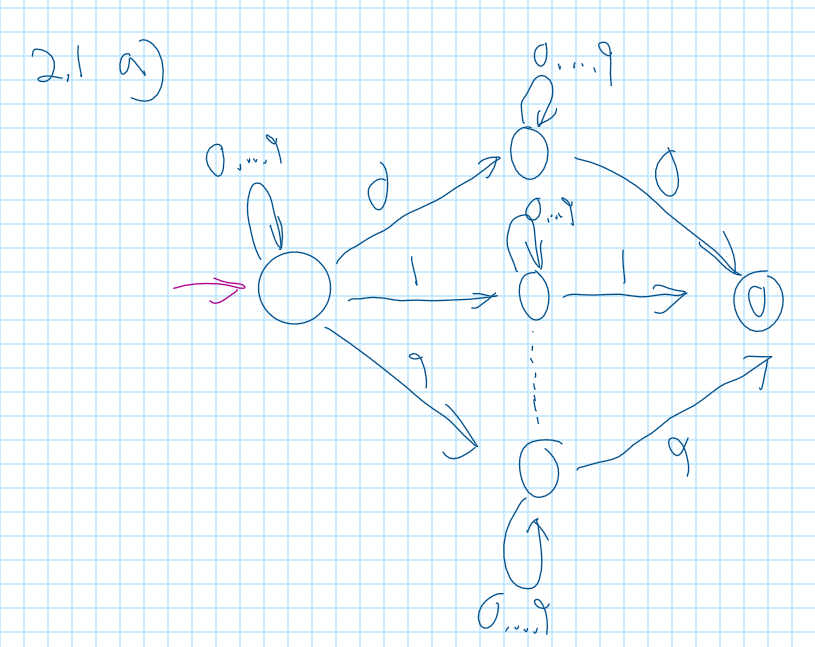
\includegraphics[scale=0.5]{Diagram 2-1-1a.png}
\end{center}

Included in my diagram is the following definition for some of the notation.
\begin{center}
    Where $\Sigma := \{0+1+2+3+4+5+6+7+8+9\}$ 
\end{center}

The regular expression for part A of exercise 2.3.4 is as follows:
\begin{center}
    \textit{( 0 + ... 9) * ( 0 ( 0 + ... 9 ) * 0 + ... )}
\end{center}
(We had gone over this in class.) The "..." is used to simplify and shorten the writing of the expression rather than writing all the digits 0 through 9.
\\
I used the "..." as a way to simplify the diagram and make it more readable by not writing every state, but enough to understand the diagram. 
The idea of the NFA is to ensure that the only way to reach the success state is to have crossed over the last digit before. 
The most helpful part for my understanding was to look at the transition to the success state has the same condition as the transition to the mid-state. 
This ensures that the digit has been seen before in the string.\\
\\
\textbf{Part B:}\\
The NFA I created is outlined in the diagram below.
\begin{center}
    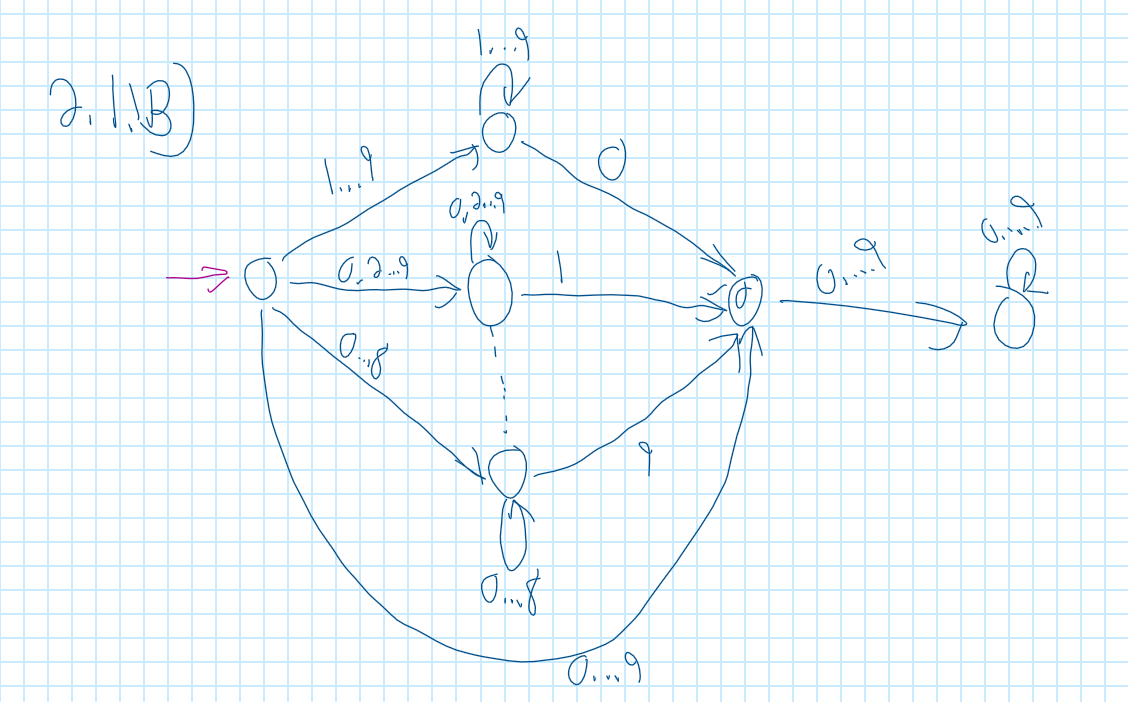
\includegraphics[scale=0.45]{Diagram 2-1-1b.png}\\
    Where $\{1-9\}:= 0+1+2+3+4+5+6+7+8+9$ \\
    $\epsilon ::= \{1-9\}*0 + \{0,2-8\}*1+...\{0-8\}*9$
\end{center}

The regular expression for part B of exercise 2.3.4 is as follows:
\begin{center}
    \textit{( 1 + ... 9 ) * 0  + ( 0 + 2 + ...9 ) * 1 + ( 0 + 1 + 3 + ...9 ) * 2 + .... (0 + ...8 ) * 9 + \textepsilon }
\end{center}
This regular expression gets all the strings where the last digit has no appeared before in the string.
\\
The main idea of this NFA is to ensure that the only way to reach the success state is to have never seen the last digit before in the string.
The part that helped me understand this NFA the most is knowing that it is effectively the complement of part A. 
So to accomplish this, I used the same foundation as the one from part A, but the transitions from the initial state are all digits except the one I'm looking for. For example, the top path is only successful if the final digit is zero, so the first transition includes all numbers 1 through 9, to prevent the possibility of 0 being seen elsewhere in the string. In addition to this, I added another state after the success to prevent the success state from firing if the transition is taken before the end of the string.\\
\\
\textbf{Part C:}\\
The NFA I created is outlined in the diagram below.
\begin{center}
    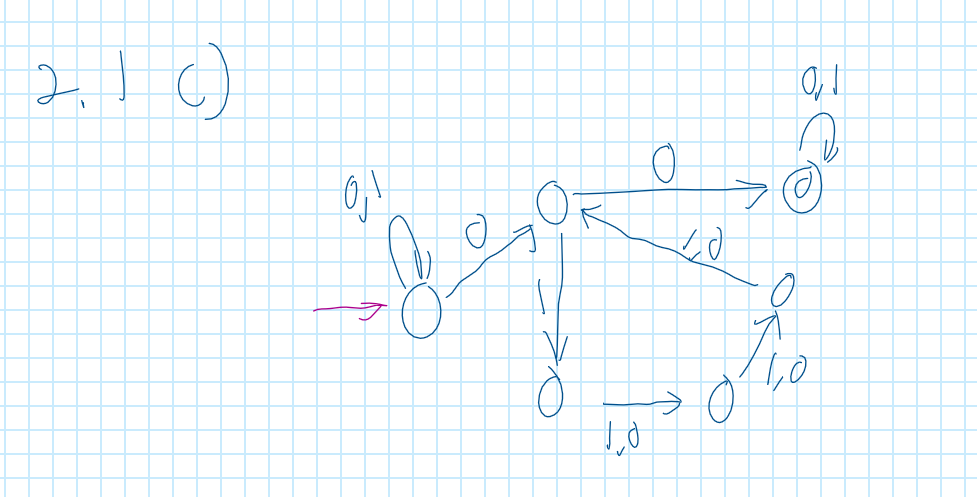
\includegraphics[scale=0.5]{Diagram 2-1-1c.png}
\end{center}
The regular expression for part C of exercise 2.3.4 is as follows:
\begin{equation}
    (0+1)^*\ 0\ ((0+1)^4)^*\ 0\ (0+1)^*
\end{equation}
For this problem, I needed some help. I utilized the website \href{https://regex101.com/}{Regex101} to help me create this regular expression. Since the above expression is not directly applicable in most programming languages, the regular expression I came up with in Regex is this:" \textit{.* 0 ((0\textpipe1)\{4\})* 0 .*} ".
\\
The main challenge with this problem is to count multiples of 4, including 0. 
I tackled this challenge by having 3 states with 4 transitions that effectively "count" the digits between 0's.
Since the problem states that the entire string doesn't have to be encased by the 0's, I have loops on the initial and success states that enable the NFA to count an entire word that contains the 0's.\\
\\
\textbf{Exercise 2.5.3}\\
Part 2 of this assignment is to answer the following questions:\\
\\
Find \textepsilon-NFAs that recognize:\\
\includegraphics[scale=0.6]{Questions 2-5-3.png}\\
\\
\textbf{Part A:}\\
The NFA that I created is outlined in the diagram below.
\begin{center}
    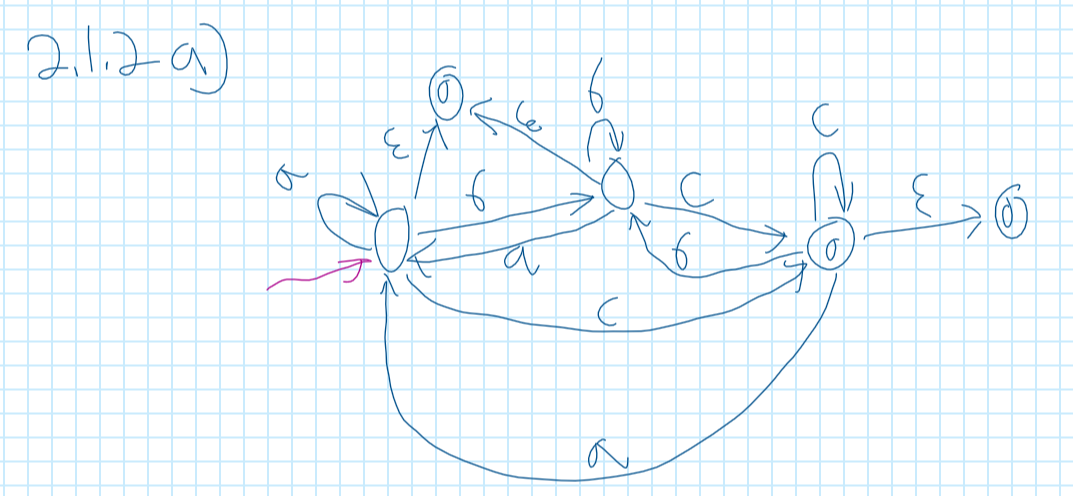
\includegraphics[scale=0.5]{Diagram 2-1-2a.png}
\end{center}
The main challenge with this NFA is the fact that there can be zero of each character. This diagram gets complex very quickly because we are looking for a pattern of alphabetical strings, but there is no guarantee that it will contain an 'a', 'b', or 'c'.
While solving this problem, there was some confusion around the phrase "consisting of." I chose to take that similar to "having substrings of" rather than "being entirely made of." If it meant "a string entirely made of a's, b's, and c's in alphabetical order", then the diagram would be slightly different and less complex.\\

\textbf{Part B:}\\
The NFA that I created is outlined in the diagram below.
\begin{center}
    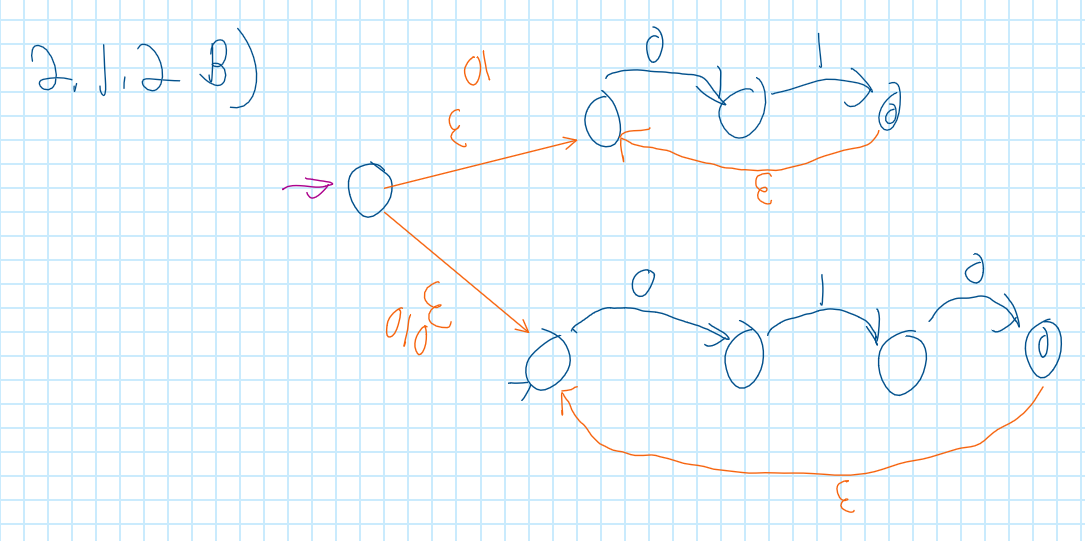
\includegraphics[scale = 0.5]{Diagram 2-1-2b.png}
\end{center}
This problem had "composition" written all over it. From the start, I noticed that this would be two automata working in parallel. 
The top section is what identifies the "01" repeating pattern while the bottom section identifies the "010" pattern. 
To "join" these two sections, I performed epsilon jumps to the beginning of each section immediately from the initial state.
To simplify the possibility of a repeating pattern, I simply jump from the success states back to that section's starting state.\\

\textbf{Part C:}\\
The NFA that I created is outlined in the diagram below.
\begin{center}
    \includegraphics[scale = 0.5]{Diagram 2-1-2c.png}
\end{center}
The main challenge with this problem was figuring out how to count 10 positions from the last. If I were implementing this program, I would simply iterate from the back of the string rather than the start, but we are unable to do that with our current setup. 
To overcome this, I created a loop of both 0's and 1's on the initial state to allow for strings longer than 10.
I then have 9 states (10 transitions) that upon finding a 1, enter the success state. If one of those states finds a 0, it will simply move onto the next position.\\

% \subsubsection{Homework 2.2.1 Regular Expressions}
% The homework discussed in this section can be found \href{https://hackmd.io/@alexhkurz/S1EVYe7bO}{here}.\\
% This homework was to write regular expressions for the languages in exercises 2.3.4 and 2.5.3 (the problems from the previous homework).\\
% \textbf{Exercise 2.3.4}\\
% \textbf{Part A:}
% The regular expression for part A of exercise 2.3.4 is as follows:
% \begin{center}
%     \textit{( 0 + ... 9) * ( 0 ( 0 + ... 9 ) * 0 + ... )}
% \end{center}
% (We had gone over this in class.) The "..." is used to simplify and shorten the writing of the expression rather than writing all the digits 0 through 9.

% \textbf{Part B:}
% The regular expression for part B of exercise 2.3.4 is as follows:
% \begin{center}
%     \textit{( 1 + ... 9 ) * 0  + ( 0 + 2 + ...9 ) * 1 + ( 0 + 1 + 3 + ...9 ) * 2 + .... (0 + ...8 ) * 9 + \textepsilon }
% \end{center}
% This regular expression gets all the strings where the last digit has no appeared before in the string.

% \textbf{Part C:}
% The regular expression for part C of exercise 2.3.4 is as follows:
% \begin{equation}
%     (0+1)^*\ 0\ ((0+1)^4)^*\ 0\ (0+1)^*
% \end{equation}
% For this problem, I needed some help. I utilized the website \href{https://regex101.com/}{Regex101} to help me create this regular expression. Since the above expression is not directly applicable in most programming languages, the regular expression I came up with in Regex is this:" \textit{.* 0 ((0\textpipe1)\{4\})* 0 .*} ".

\textbf{Exercise 2.5.3}\\
\textbf{Part A:}\\
The regular expression for part A is as follows:
\begin{center}
   \textit{a* b* c*}
\end{center}
This was was very simple because the * is what allows the preceding character to appear anywhere between 0 and unlimited number of times.\\

\textbf{Part B:}\\
The regular expression for part B is as follows:
\begin{center}
    \textit{(01)(01)* + (010)(010)*}
\end{center}
For this problem, I needed some help again. The regular expression I came up with in Regex101 is this: \textit{(01)(01)+\ \textpipe\ (010)(010)+}\\

\textbf{Part C:}\\
The regular expression for part C is as follows:
\begin{equation}
    (0+1)^* 1 (0+1)^n\ ,\ where\ 0 <= n <= 9
\end{equation}

Since this question says that the number 1 must appear in the last 10 digits and we have the ability to use exponents in our definition, I'm using N as a way to ensure that the 1 can show up anywhere in the last 10 positions. I also had some help from \href{https://regex101.com/}{Regex101} for this problem and the equivalent expression I got in Regex101 while I was working on this problem was " \textit{.* 1 (1\textpipe0)\{0,9\}\$} ".

\subsection{Week 3}
\subsubsection{Homework 3.1 Converting NFAs to DFAs}
The homework discussed in this section can be found \href{https://hackmd.io/@alexhkurz/HylLKujCP}{here}.\\
\textbf{Exercise 2.3.1}\\
Part 1 of this assignment is to answer the following question:
\begin{center}
    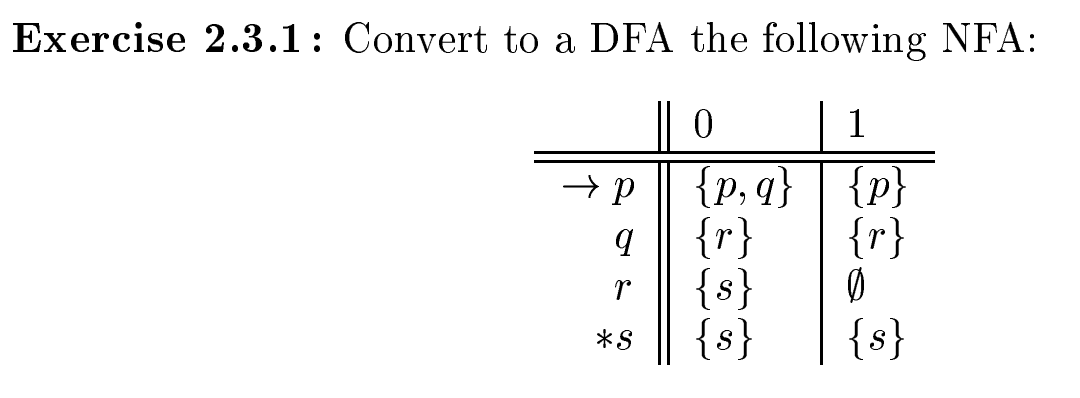
\includegraphics[scale=0.25]{Question231Chart.png}
\end{center}

The diagram for the DFA can be found below:
\begin{center}
    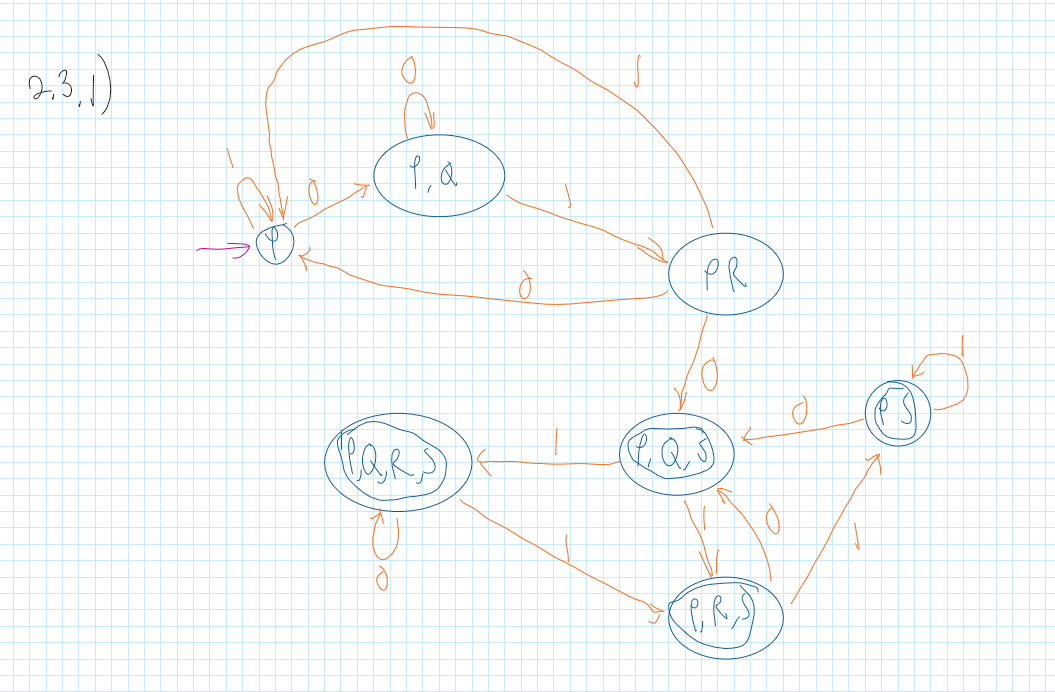
\includegraphics[scale=0.55]{Diagram 2-3-1 DFA.png}
\end{center}
\\
\textbf{Exercise 2.3.2}
Part 2 of this assignment is to answer the following question:
\begin{center}
    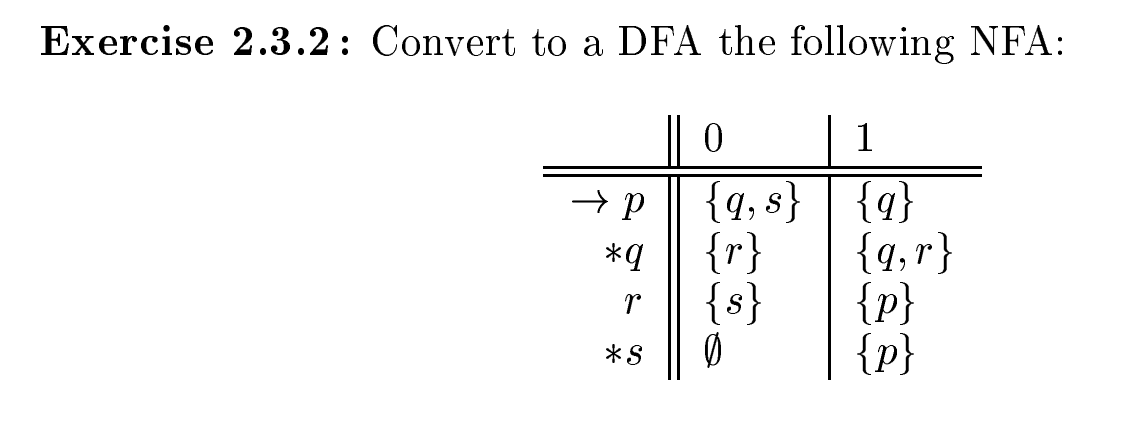
\includegraphics[scale=0.25]{Question232Chart.png}
\end{center}

The diagram for the DFA can be found below:
\begin{center}
    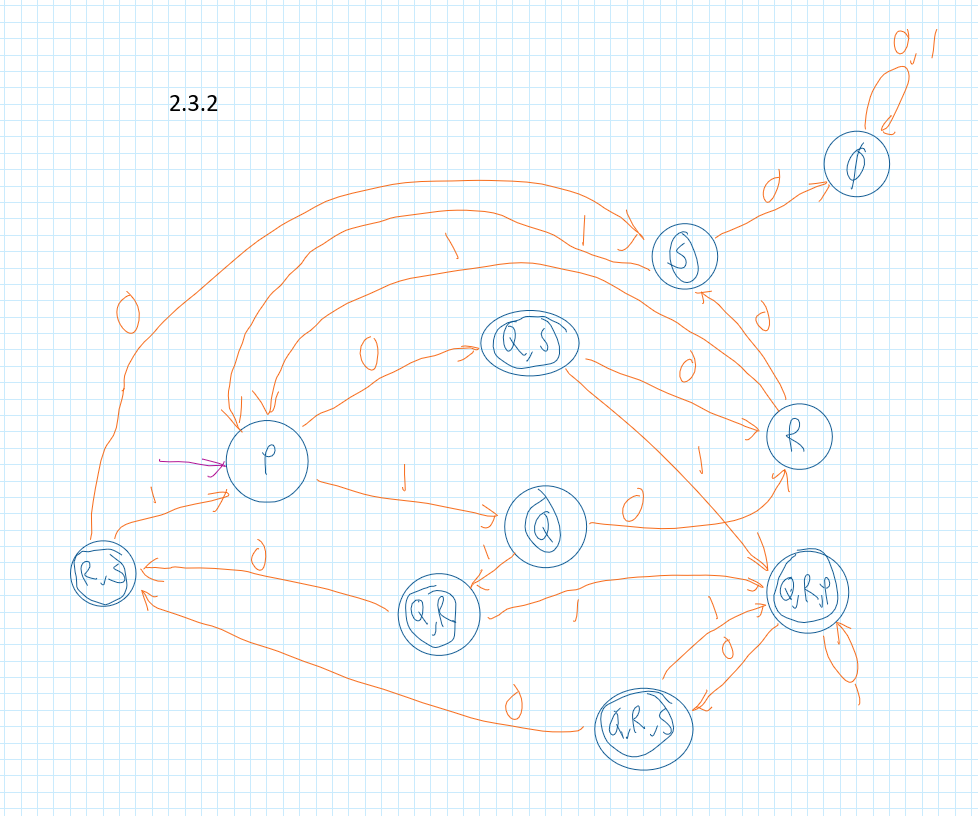
\includegraphics[scale=0.5]{Diagram 2-3-2 DFA.png}
\end{center}
\\
\textbf{Exercise Converting NFAs to DFAs in Haskell}

Part 2 of this assignment is to complete the following task:
\begin{center}
"Put the definitions of dfa\_initial, dfa\_final, dfa\_delta in the report and explain your code in a paragraph. Also put your modified version of automata05.hs in your github repository.)

The file automata05 provides a template, in which you have to modify lines 71, 72, 73. Complete the definition of nfa2dfa as described in the three bullet points above and test it with various examples."
\end{center}

My code can be seen below:

\begin{lstlisting}[language=Haskell]
-- convert an NFA to a DFA
nfa2dfa :: NFA s -> DFA [s]
nfa2dfa nfa = DFA {
  -- exercise: correct the next three definitions 
  dfa_initial = [nfa_initial nfa],
  --dfa_final = let final qs = True in final,
  dfa_final = 
   let 
    --final var1 var2 = (var1 var2)
    --final nfa = disjunction nfa
    --final 
    --final [s] = disjunction(nfa_final s)
        --final (q:qs) = final qs
      --final var1 = (final (nfa_final var1))
      --final qs = [nfa]
      final qs = map (disjunction) (qs)
      


   in final,
  dfa_delta = 
   let 
    delta qs c = qs 
    --delta [] c = 
    --delta (q:qs) c = 
   in delta }
\end{lstlisting}

Sadly, I was unable to complete this section. I am confident in my answer for dfa\_initial, but I'm far from confident for dfa\_final and dfa\_delta. 
I tried to comment all of my attempts in order to show the many thought processes I had. 
I also hope that one of them was close. I think the hardest part for me was understanding the data types of all of the variables and knowing what was being passed into the function in the first place. 
I was really struggling with understanding how to use what felt like Object Oriented Programming inside of a functional language. 

\subsection{Week 4}
The homework for week 4 can be found \href{https://hackmd.io/@alexhkurz/HJ4KjezfO}{here}.\\
Both parts of this assignment involved the code for C--, and that can be found \href{https://github.com/alexhkurz/compiler-construction-2022/blob/main/bnfc-tutorial-C--.md}{here}.\\

The point of the homework was to create concrete and abstract syntax trees for the basic program in C--. 
My Concrete Syntax Tree can be found below. To get a better look, \href{https://github.com/mamba72/CompilerConstruction_Assignments/blob/main/Reports/ReportResources/4-1\%20Full\%20Concrete\%20Syntax\%20Tree.png}{here is a link to the photo on GitHub}.\\
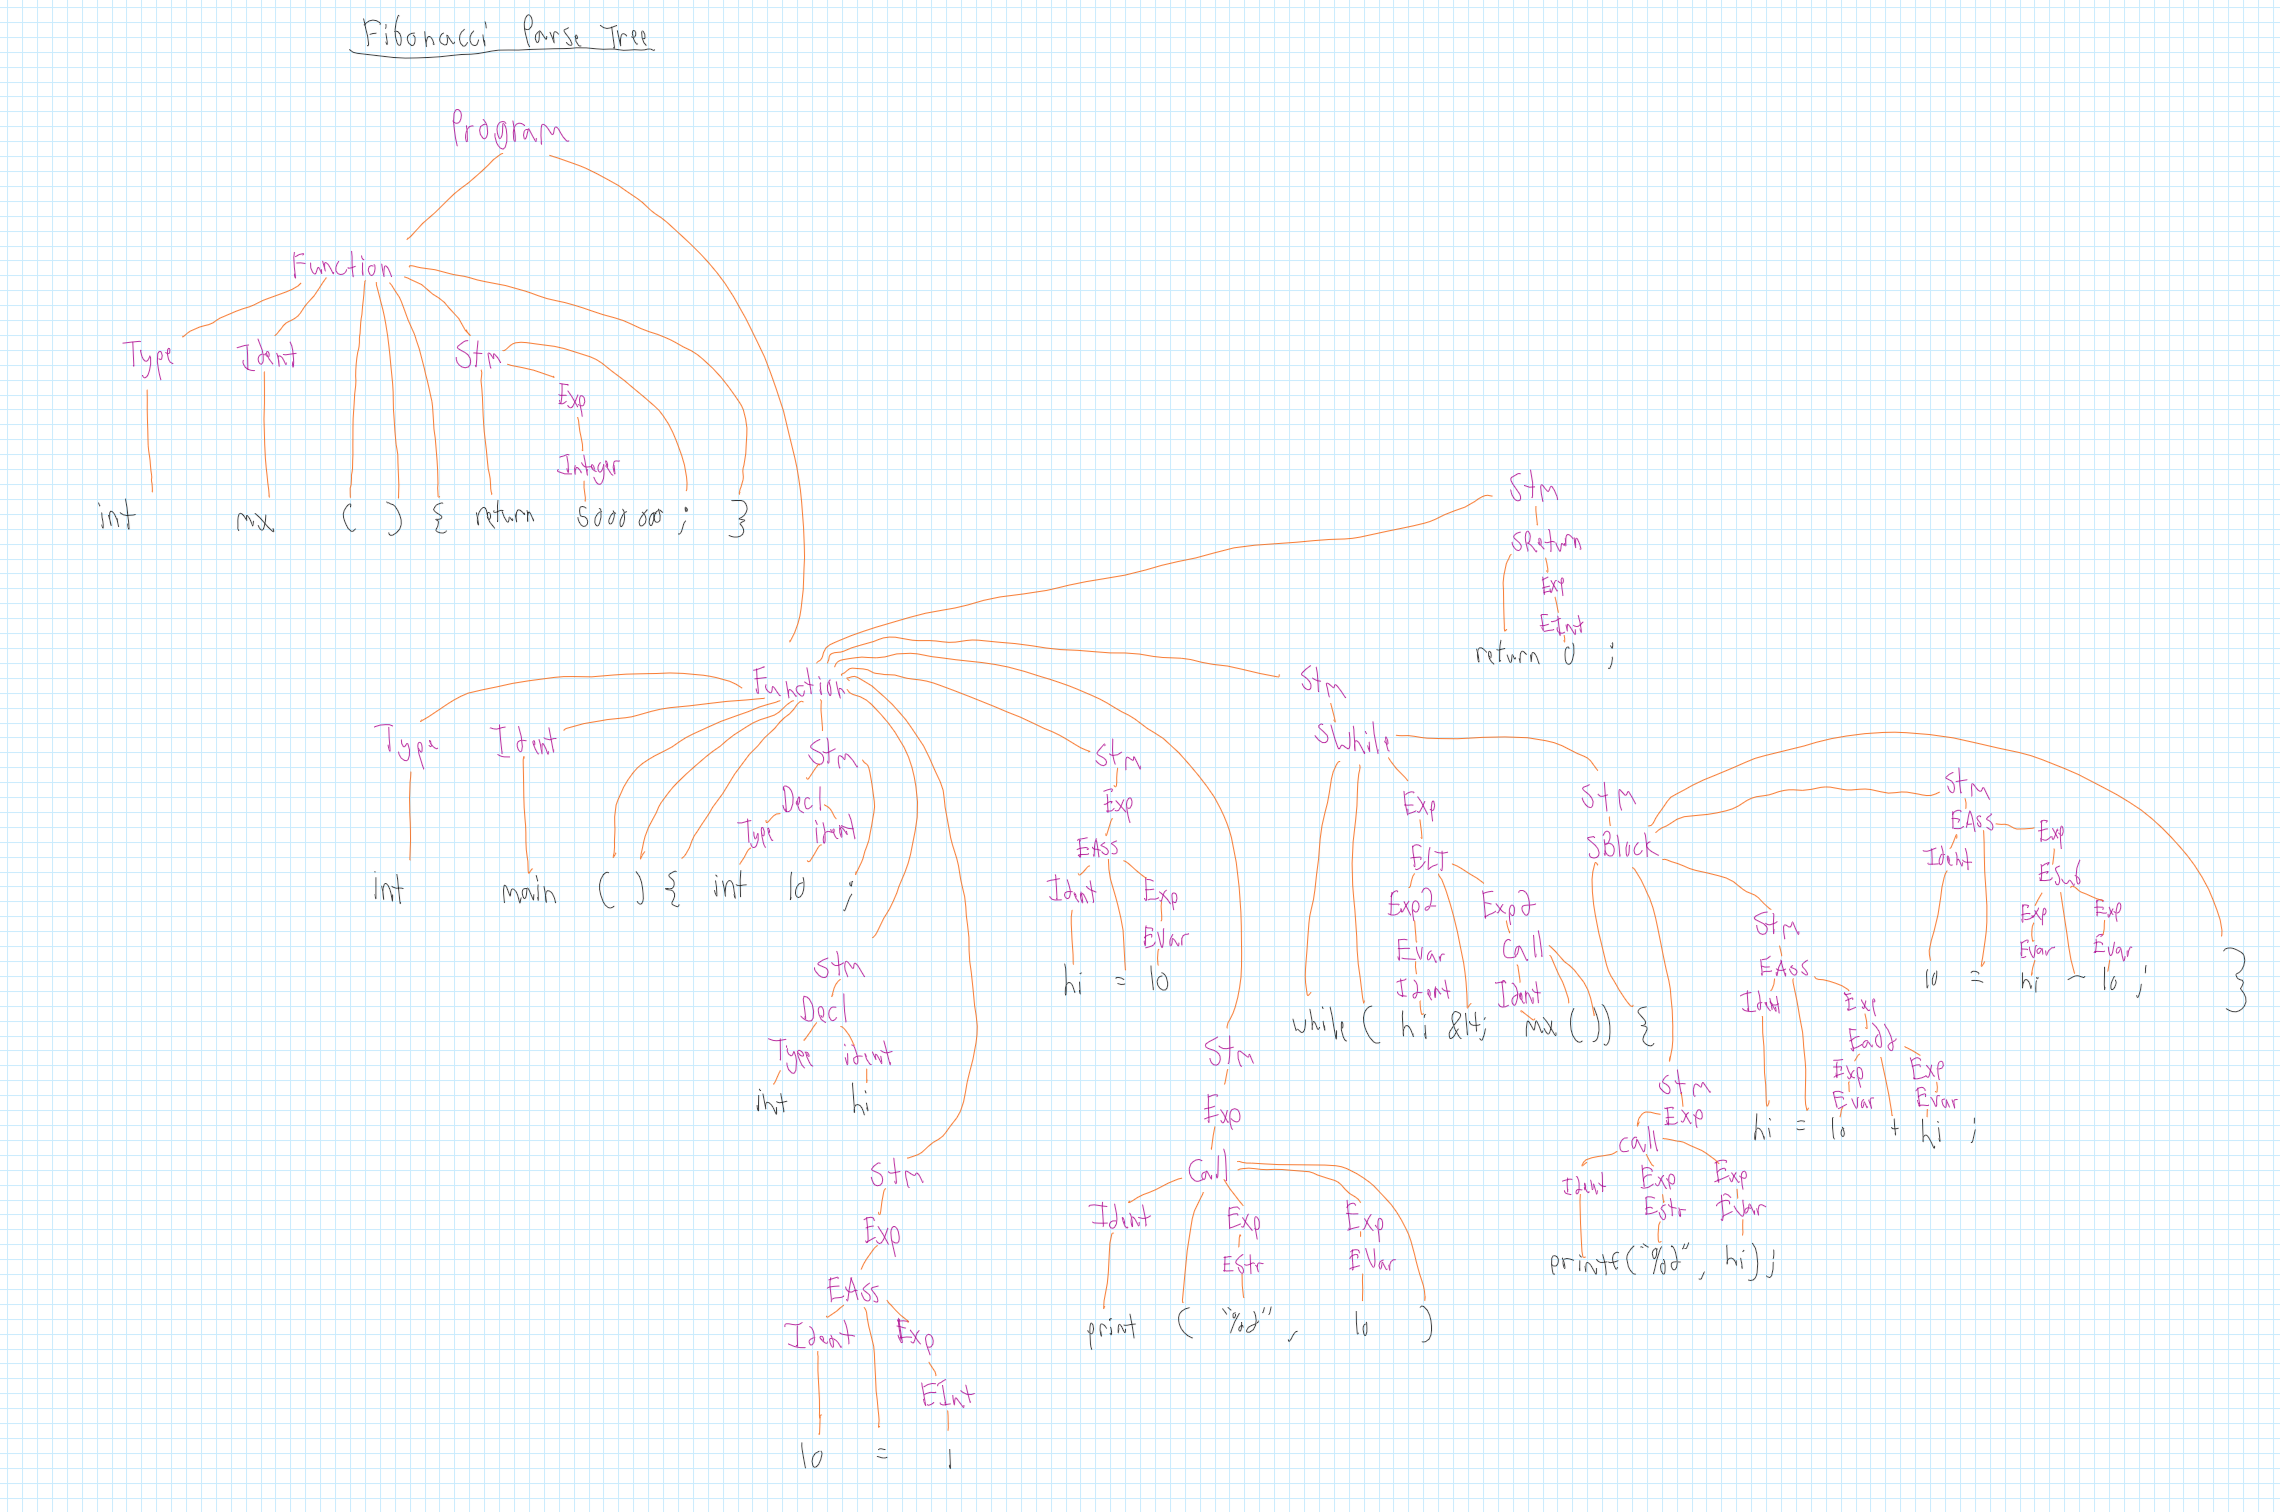
\includegraphics[scale=0.315]{4-1 Full Concrete Syntax Tree.png}\\
\\
My Abstract Syntax Tree can be found below. To get a better look, \href{https://github.com/mamba72/CompilerConstruction_Assignments/blob/main/Reports/ReportResources/4-1\%20Full\%20Abstract\%20Syntax\%20Tree.png}{here is a link to the photo on GitHub}.\\
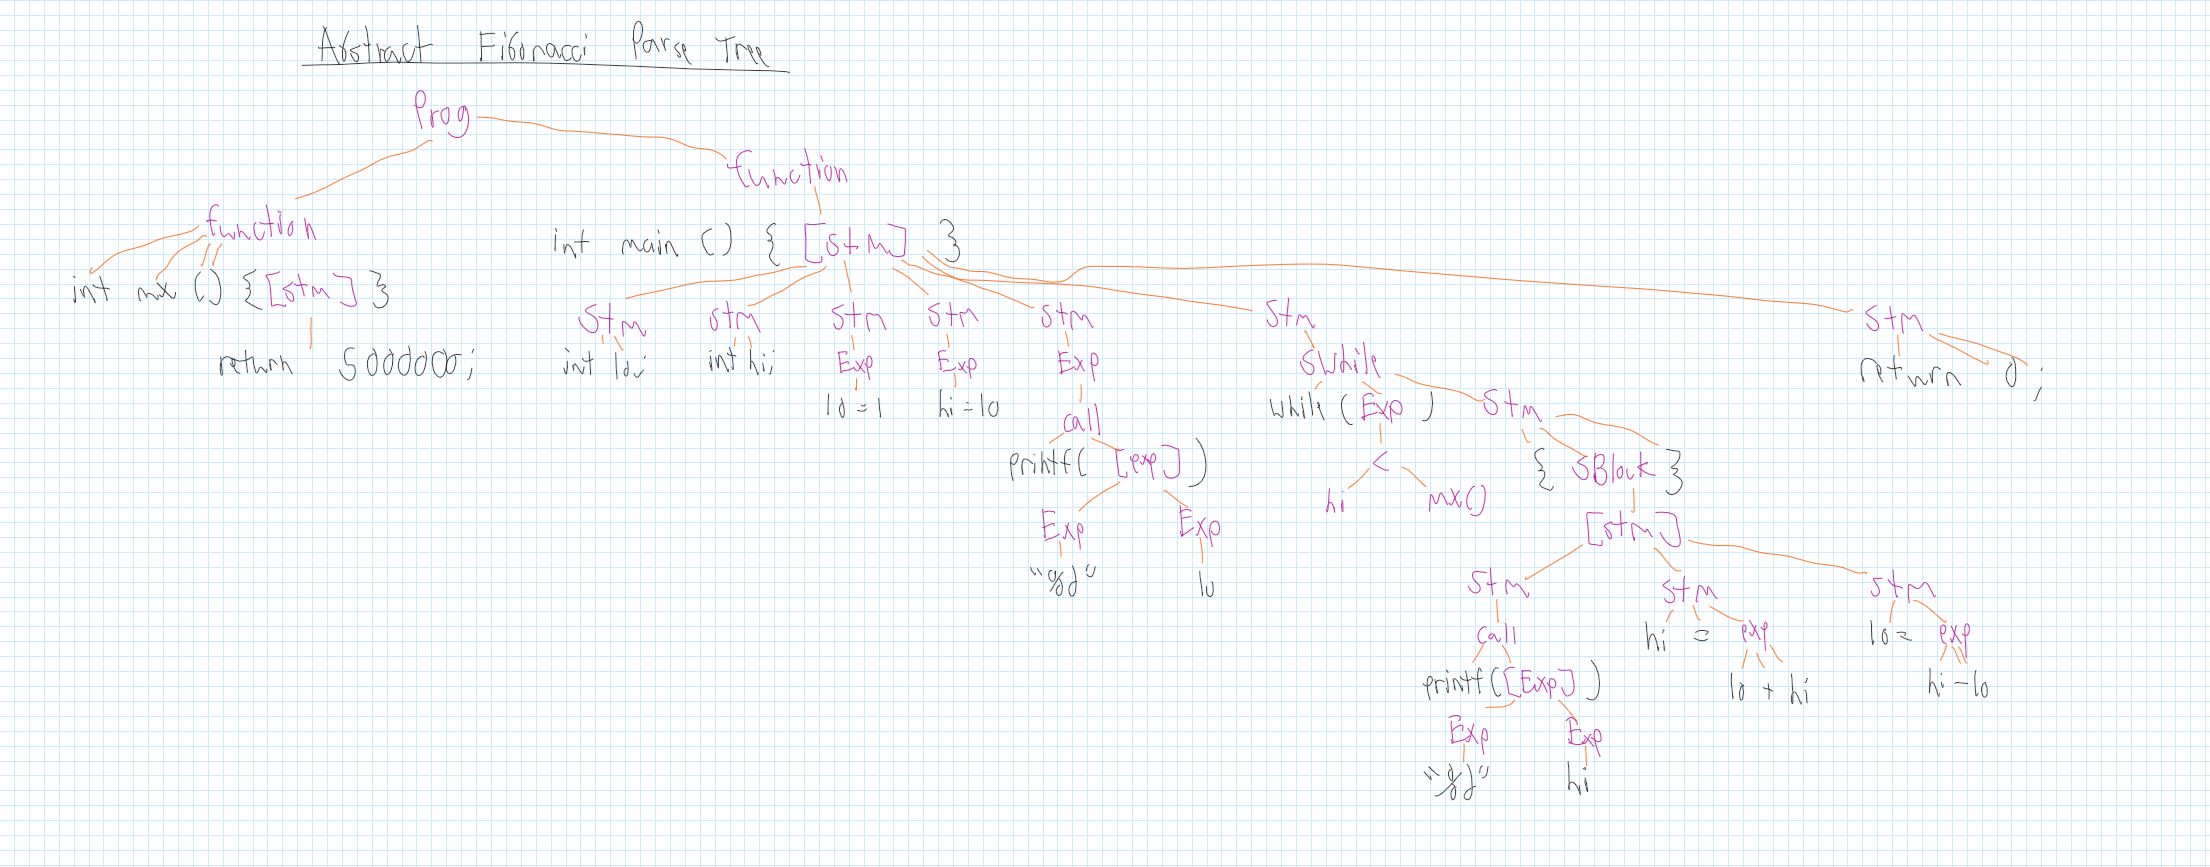
\includegraphics[scale=0.35]{4-1 Full Abstract Syntax Tree.png}\\

\section{Project}

\subsection{Initial Project Description}
For the project, I will be using C as my programming language and I will be using the GCC compiler to compile it to Assembly. My C program will simply be a hard coded number and printing out the factorial of that number. My C program can be found \href{https://github.com/mamba72/CompilerConstruction_Assignments/blob/main/ExplainingACompiler/CProgram.c}{here}. My Assembly can be found \href{https://github.com/mamba72/CompilerConstruction_Assignments/blob/main/ExplainingACompiler/CProgram.out}{here}.

\begin{lstlisting}{language=C}
        #include <stdio.h>

        //Created a program does factorial
        int main()
        {
            int num = 3;
        
            int product = 1;
        
            while(num > 0)
            {
                product *= num;
        
                num = num - 1;
            }
        
            printf("Product:",product);
        
            return 0;
        }
\end{lstlisting}

The following is the GCC assembly Output.

\begin{lstlisting}{language=Assembly}
    	.file	"CProgram.c"  --> This line says where the program came from
        	.text --> This tells what encoding the file is in
        	.globl	main --> This says that the "main" pointer is global.
        	.type	main, @function --> This says that the "main" pointer points to a function
        main: --> this is the label for the beginning of the main function
        .LFB0: --> this is the label for the opening bracket in the main function
        	.cfi_startproc --> used in debugging. Initializes internal data structures allowing the function to be in the .eh_frame 
        	endbr64 --> inserts a NOP into the pipeline to prevent data hazards or corruption.
        	pushq	%rbp --> this pushes a new context onto the stack because we entered a new code block.
        	.cfi_def_cfa_offset 16 --> Changes the absolute offset that will be added to a defined register to compute the CFA address
        	.cfi_offset 6, -16 --> the previous value of register 6 is saved at the offset -16 from the CFA pointer.
        	movq	%rsp, %rbp --> memory copies the base point value into stack pointer reference, giving it a reference for where it is in memory.
        	.cfi_def_cfa_register 6 --> will now use register 6 instead of the old CFA register. Offset is unchanged.
        	subq	$16, %rsp --> integer subtraction. Moving the current pointer to show that we are in a new statement block.
        	movl	$3, -4(%rbp) --> initializing the value of 3 into a new "num" variable. ("num" = -4(%rbp))
        	movl	$1, -8(%rbp) --> initializing the value of 1 into a new "product" variable. ("product" = -8(%rbp))
        	jmp	.L2 --> an unconditional jump to label L2
        .L3: --> label L3. This is the inside of the while loop.
        	movl	-8(%rbp), %eax --> this is putting the value of product into the register EAX as a temporary variable.
        	imull	-4(%rbp), %eax --> Integer Multiplication. this is multiplying num by the temporary value in the register.
        	movl	%eax, -8(%rbp) --> this is copying the new value of (product' * num) into the register for product.
        	subl	$1, -4(%rbp) --> integer subtraction. Subtracting 1 from num in place.
        .L2: --> label L2
        	cmpl	$0, -4(%rbp) --> This is the condition in the while loop. Checks if "num" is greater than 0.
        	jg	.L3 --> conditional jump when "num" > 0 is true. If true, it will enter the while.
        	--> if we reached here, we are outside the while loop.
        	movl	-8(%rbp), %eax --> this is putting the value of product into the register EAX as a temporary variable.
        	cltq    --> converting integer into a Long for printing.
        	movq	%rax, %rdi --> Puts the literal string "Product" onto the stack so it can be an argument in the printf function.
        	movl	$0, %eax --> EAX is expected to hold the number of vector registers for the printf arguments, but we are simply printing an integer, so there is no need for a vector register.
        	call	printf@PLT --> calls the printf function.
        	movl	$0, %eax --> puts a 0 into the EAX register for the return statement.
        	leave --> leaves the current statement block
        	.cfi_def_cfa 7, 8 --> changing offset for the CFA register 7.
        	ret --> returning from the subroutine.
        	.cfi_endproc --> The ending to the .cfi_startproc to signify the end of the function to the debugger.
        .LFE0: --> this is the section that helps the system handle exceptions and adds information for the debugger.
        	.size	main, .-main
        	.ident	"GCC: (Ubuntu 9.3.0-17ubuntu1~20.04) 9.3.0"
        	.section	.note.GNU-stack,"",@progbits
        	.section	.note.gnu.property,"a"
        	.align 8
        	.long	 1f - 0f
        	.long	 4f - 1f
        	.long	 5
        0:
        	.string	 "GNU"
        1:
        	.align 8
        	.long	 0xc0000002
        	.long	 3f - 2f
        2:
        	.long	 0x3
        3:
        	.align 8
        4:

\end{lstlisting}



\section{Homework Continued}
\subsection{Week 10}
\subsubsection{Creating a Proof Tree}
The instructions for this assignment can be seen \href{https://hackmd.io/@alexhkurz/SkZELd3X5}{here}.
The point of this assignment was to create the tree of steps the interpreter would take while completing the following program:

\begin{lstlisting}

int x;
{
    x = 2 ;
    bool x = false && x ;
    y = y++ + ++y ;
}
x = y ;

\end{lstlisting}


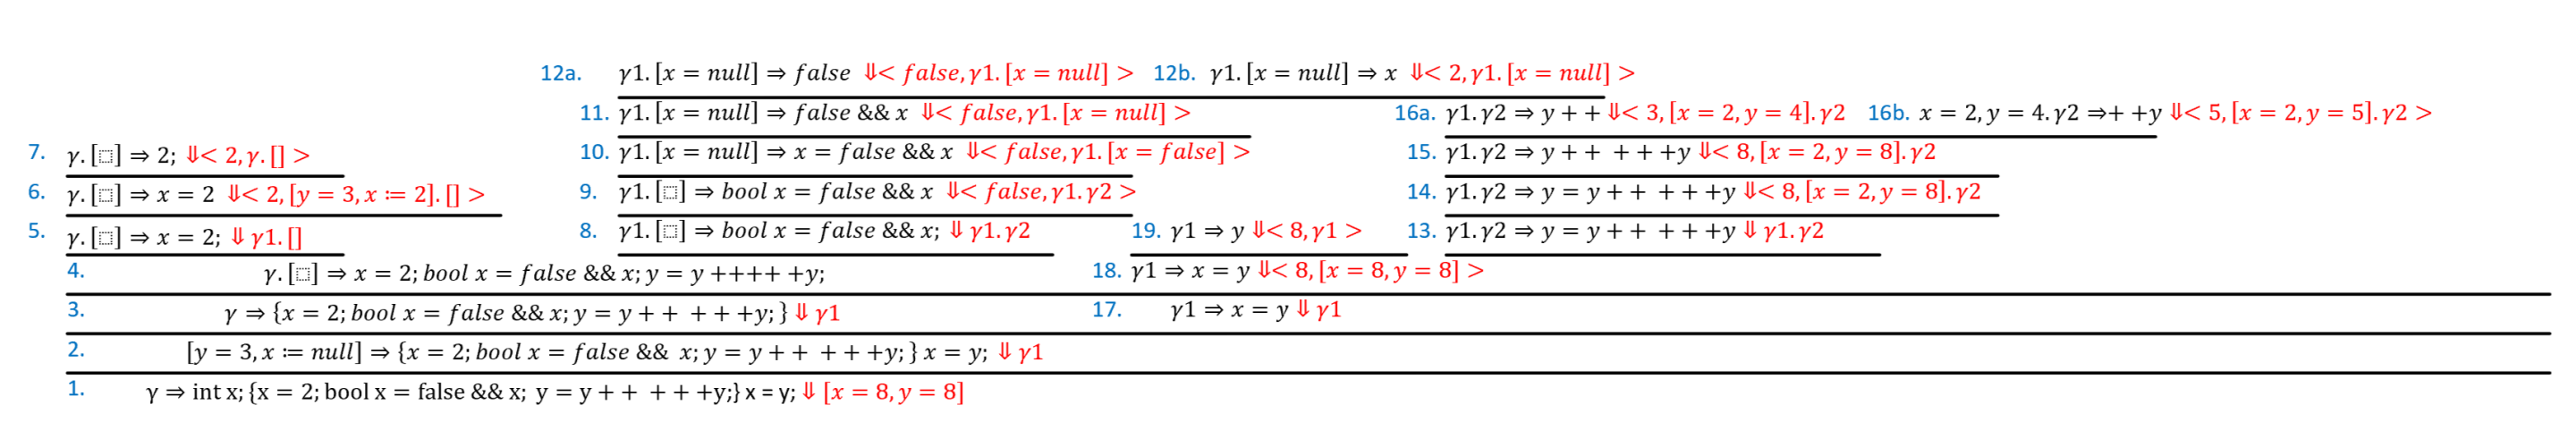
\includegraphics[scale=0.18]{ProofTree.png}

\begin{enumerate}
    \item\begin{prooftree} % 1. declaration
            \AxiomC{}
            \UnaryInfC{$\gamma \rightarrow  T x; \downarrow \gamma(x := null)$}
        \end{prooftree}
    \item\begin{prooftree} % 2. interpretation of statements
            \AxiomC{$\gamma \rightarrow s \downarrow \gamma`$}
            \AxiomC{$\gamma` \rightarrow S2...Sn\downarrow \gamma``$}
            \BinaryInfC{$\gamma \rightarrow S1...Sn \downarrow \gamma``$}
        \end{prooftree}
    \item \begin{prooftree} % 3. block statements
            \AxiomC{$\gamma. \rightarrow S1...Sn \downarrow \gamma`.\delta$}
            \UnaryInfC{$\gamma \rightarrow \{S1...Sn\} \downarrow \gamma`$}
        \end{prooftree}
    \item \begin{prooftree} % 4. interpretation of statements
            \AxiomC{$\gamma \rightarrow s \downarrow \gamma`$}
            \AxiomC{$\gamma` \rightarrow S2...Sn\downarrow \gamma``$}
            \BinaryInfC{$\gamma \rightarrow S1...Sn \downarrow \gamma``$}
        \end{prooftree}
    \item \begin{prooftree} % 5. going from expression to statement
            \AxiomC{$\gamma \rightarrow e \downarrow <v,\gamma`> $}
            \UnaryInfC{$\gamma \rightarrow e; \downarrow \gamma`$}
        \end{prooftree}
    \item \begin{prooftree} % 6. assignment rule
            \AxiomC{$\gamma \rightarrow e \downarrow <v,\gamma`> $}
            \UnaryInfC{$\gamma \rightarrow x=e \downarrow <v,\gamma`(x:=v)>$}
        \end{prooftree}
    \item \begin{prooftree} % 7. lookup
            \AxiomC{}
            \UnaryInfC{$\gamma \rightarrow x \downarrow v$}
        \end{prooftree}
    \item \begin{prooftree} % 8. going from expression to statement
            \AxiomC{$\gamma \rightarrow e \downarrow <v,\gamma`> $}
            \UnaryInfC{$\gamma \rightarrow e; \downarrow \gamma`$}
        \end{prooftree}   
    \item\begin{prooftree} % 9. declaration
            \AxiomC{}
            \UnaryInfC{$\gamma \rightarrow  T x; \downarrow \gamma(x := null)$}
        \end{prooftree}
    \item\begin{prooftree} % 10. assignment rule
            \AxiomC{$\gamma \rightarrow e \downarrow <v,\gamma`> $}
            \UnaryInfC{$\gamma \rightarrow x=e \downarrow <v,\gamma`(x:=v)>$}
        \end{prooftree}
    \item\begin{prooftree} % 11. AND rule
            \AxiomC{$\gamma \rightarrow a \downarrow u$}
            \AxiomC{$\gamma \rightarrow b \downarrow v$}
            \BinaryInfC{$\gamma \rightarrow a\&\&b \downarrow u\ x\ v$}
        \end{prooftree}
    \item\begin{prooftree} % 12a. lookup
            \AxiomC{}
            \UnaryInfC{$\gamma \rightarrow x \downarrow v$}
        \end{prooftree}
    \item\begin{prooftree} % 13. going from expression to statement
            \AxiomC{$\gamma \rightarrow e \downarrow <v,\gamma`> $}
            \UnaryInfC{$\gamma \rightarrow e; \downarrow \gamma`$}
        \end{prooftree}
    \item\begin{prooftree} % 14. assignment rule
            \AxiomC{$\gamma \rightarrow e \downarrow <v,\gamma`> $}
            \UnaryInfC{$\gamma \rightarrow x=e \downarrow <v,\gamma`(x:=v)>$}
        \end{prooftree}
    \item\begin{prooftree} % 15. addition rule
            \AxiomC{$\gamma \rightarrow x \downarrow v $}
            \AxiomC{$\gamma \rightarrow x \downarrow v $}
            \BinaryInfC{$\gamma \rightarrow a + b \downarrow <v,\gamma`>$}
        \end{prooftree}
    \item\begin{prooftree} % 16. Post and Pre Increment
            \AxiomC{}
            \UnaryInfC{$\gamma \rightarrow x++ \downarrow <v,\gamma`(x:=v+1)>$}
        \end{prooftree}
    \item\begin{prooftree} % 17. Expression to Statement
            \AxiomC{$\gamma \rightarrow e \downarrow <v,\gamma`> $}
            \UnaryInfC{$\gamma \rightarrow e; \downarrow \gamma`$}
        \end{prooftree}
    \item\begin{prooftree} % 18. Assignment
            \AxiomC{$\gamma \rightarrow e \downarrow <v,\gamma`> $}
            \UnaryInfC{$\gamma \rightarrow x=e \downarrow <v,\gamma`(x:=v)>$}
        \end{prooftree}
    \item\begin{prooftree} % 19. Assignment
            \AxiomC{}
            \UnaryInfC{$\gamma \rightarrow x \downarrow v$}
        \end{prooftree}
    
\end{enumerate}



\section{Conclusions}\label{conclusions}

%(approx 400 words)

%In the conclusion, I want a critical reflection on the content of the course. Step back from the technical details. How does the course fit into the wider world of programming languages and software engineering?

To make a poor analogy, this course is like a construction worker learning physics. Technically, a builder can put a building together and follow the instructions on the blueprints without knowing why the engineer did any of it. The problem with the builder working like that is he has no way of utilizing his building skills without someone telling him what to build. This is analogous to the life of a software engineer because yes, technically any 12-year-old can create a basic video game in python by following a YouTube tutorial, but there is so much more to programming than following instructions. 
\\\\
This course allows us to go from basically utilizing the tools provided to us to being able to create our own tools to better tackle the next problem we face. In my life this has been made very clear through talking to my dad about the problems he faces on the day to day. My dad is a UCLA graduate with a degree in computer science and he said that Compiler Construction is the most useful class he’s taken. In his work, he created a parser to automatically extract information from and categorize his employer’s mess of custom stock trade orders. As I took this class, we were able to talk more and more about how his parser works and why he does what he does. I am able to understand the problems he faces and how I might be able to tackle the same solutions. 
\\\\
This class was also incredibly effective at teaching me how to use the basic tools to create more complex ones. This class hammers recursion into our brains. Recursion has always been an incredibly challenging topic for me. Challenging to create. Challenging to debug. Challenging to read. This class has taught me how to approach recursion and the kinds of problems that can best be overcome using recursion. 
\\\\
This class is a fantastic class to follow up from taking Computer Architecture my previous semester. Over the years I’ve been learning about how to create software and how to build solutions, but I never understood how a computer actually worked. I finally took Computer Architecture and then I was still left with questions. Thankfully less questions, but still questions. The biggest one was “so I can build software solutions and I know how we turned a chunk of silicon into a fancy math machine… now how does my code get to the assembly for the computer?” This class has now filled in the whole stack. From keyboard stroke to transistor, I have an (admittedly a general and high level) understanding of every step in between. 
\\\\
I think this class has allowed me to better understand the strange quirks and mishaps that occur when programming. I am far more knowledgeable on why some syntax just doesn’t work. I am far more capable of predicting what certain code will do before I run it, because I now (at least mostly) understand how it is actually being computed. As a software engineer, I am now able to better understand the tools at my disposal, and I am able to better apply myself to any problem. I’ve graduated from the builder to the engineer, the programmer to the software engineer.


% \begin{thebibliography}{99}
% \bibitem[HMU]{Hopcroft}
% 	John E. Hopcroft, Rajeev Motwani, Jeffrey D. Ullman:
% \href{http://ce.sharif.edu/courses/94-95/1/ce414-2/resources/root/Text\%20Books/Automata/John\%20E.\%20Hopcroft,\%20Rajeev\%20Motwani,\%20Jeffrey\%20D.\%20Ullman-Introduction\%20to\%20Automata\%20Theory,\%20Languages,\%20and\%20Computations-Prentice\%20Hall\%20(2006).pdf}{Introduction to automata theory, languages, and computation,} 3rd Edition. Pearson international edition, Addison-Wesley 2007


% \end{thebibliography}

\medskip

\printbibliography


\cite{noauthor_cfi_nodate}
\cite{noauthor_guide_nodate}
\cite{godbolt_compiler_nodate}
\cite{john_e._introduction_nodate}
\cite{noauthor_assembly_nodate}
\cite{noauthor_macos_nodate}
\cite{noauthor_x86_nodate-1}
\cite{noauthor_x86_nodate}


\end{document}
